\subsection{Đề 4}
\caulc
\Opensolutionfile{ans}[ans/ansCTST-1OTHK1-De4]
\begin{ex}%[1D1H5-3]
	Nghiệm của phương trình $2\cos x-1=0$ là
	\choice
	{$x=\pm \dfrac{2\pi}{3}+k2\pi,k\in \mathbb{Z}$}
	{$x=\pm \dfrac{\pi}{6}+k\pi,k\in \mathbb{Z}$}
	{\True $x=\pm \dfrac{\pi}{3}+k2\pi,k\in \mathbb{Z}$}
	{$x=\pm \dfrac{\pi}{6}+k2\pi,k\in \mathbb{Z}$}
	\loigiai{
		Ta có $2\cos x-1=0\Leftrightarrow \cos x=\dfrac{1}{2}\Leftrightarrow \cos x=\cos \dfrac{\pi}{3}\Leftrightarrow x=\pm \dfrac{\pi}{3}+k2\pi,k\in \mathbb{Z}$.
	}
\end{ex}
\begin{ex}%[1D2H3-2]
	Dãy số cho bởi công thức nào dưới đây \textbf{không} phải là cấp số nhân?
	\choice
	{$u_n=\dfrac{3^n}{2}$}
	{$u_n=\dfrac{2}{5^n}$}
	{$u_n=\left(-1\right)^n$}
	{\True $u_n=3n+2$}
	\loigiai{
		Ta có
		$u_n=\dfrac{3^n}{2}$ là số hạng tổng quát của cấp số nhân vì $\dfrac{u_{n+1}}{u_n}=3$.\\
		$u_n=\dfrac{2}{5^n}$ là số hạng tổng quát của cấp số nhân vì $\dfrac{u_{n+1}}{u_n}=\dfrac{1}{5}$.\\
		$u_n=\left(-1\right)^n$ là số hạng tổng quát của cấp số nhân vì $\dfrac{u_{n+1}}{u_n}=-1$.
	}
\end{ex}
\begin{ex}%[1D3H1-4]
	Tính $\lim \dfrac{8n^2+n-2}{n^2}$.
	\choice
	{$3$}
	{$0$}
	{$-2$}
	{\True $8$}
	\loigiai{
		Ta có $\lim \dfrac{8n^2+n-2}{n^2}=\lim \left(8+\dfrac{1}{n}-\dfrac{2}{n^2}\right)=8$.
	}
\end{ex}
\begin{ex}%[1D3H2-2]
	Giới hạn $\lim\limits_{x\to 1}\, \dfrac{x-3}{x+2}$ bằng
	\choice
	{$0$}
	{\True $\dfrac{-2}{3}$}
	{$+\infty $}
	{$1$}
	\loigiai{
		Ta có $\lim\limits_{x\to 1}\, \dfrac{x-3}{x+2}=\dfrac{1-3}{1+2}=\dfrac{-2}{2}$.
	}
\end{ex}
\begin{ex}%[1D3N3-4]
	Cho hàm số $f(x)=\dfrac{3}{x+3}$. Khẳng định nào sau đây đúng?
	\choice
	{\True Hàm số liên tục trên mỗi khoảng $(-\infty;-3)$ và $(-3;+\infty)$}
	{Hàm số liên tục trên mỗi khoảng $(-\infty;0)$ và $(0;+\infty)$}
	{Hàm số liên tục trên $\mathbb{R}$}
	{Hàm số liên tục trên mỗi khoảng $(-\infty;3)$ và $(3;+\infty)$}
	\loigiai{
		Hàm số $f(x)=\dfrac{3}{x+3}$ có tập xác định là $x+3\ne 0\Rightarrow x\ne -3$.\\
		Nên hàm số liên tục trên mỗi khoảng $(-\infty;-3)$ và $(-3;+\infty)$.
	}
\end{ex}
\begin{ex}%[1D3H3-3]
	Hàm số nào sau đây liên tục tại điểm $x_0=4$?
	\choice
	{\True $f(x)=\heva{&\dfrac{x}{3x-8} \left(x\ne 4\right) \\&1 \left(x=4\right)}$}
	{$f(x)=\dfrac{2}{x-4}$}
	{$f(x)=\heva{&x^2-13 \left(x\le 4\right) \\&\sqrt{5x+5} \left(x>4\right)}$}
	{$f(x)=\heva{&2x+5 \left(x>4\right) \\&12 \left(x\le 4\right)}$}
	\loigiai{
		Ta có $\heva{&\lim\limits_{x\to 4}\, \dfrac{x}{3x-8}=1 \\&f(4)=1}
		\Rightarrow \lim\limits_{x\to 4}\, \dfrac{x}{3x-8}=f(4)=1$ nên hàm số liên tục tại điểm $x_0=4$.
	}
\end{ex}
\begin{ex}%[1H4N4-2]
	Cho hình lập phương $ABCD.A'B'C'D'$. Chọn khẳng định đúng.
	\choice
	{\True $\left(ABCD\right)\parallel \left(A'B'D'\right)$}
	{$\left(A'D'C\right)\parallel \left(ABCD\right)$}
	{$\left(D'C'A\right)\parallel \left(ABCD\right)$}
	{$\left(BCC'B'\right)\parallel \left(ABCD\right)$}
\loigiai{
	\immini{
		Dựa vào hình vẽ của hình lập phương, ta có $\left(ABCD\right)\parallel \left(A'B'D'\right)$.
	}
	{
		\begin{tikzpicture}[scale=.7,line cap=round,line join=round,font=\footnotesize,>=stealth]
			\path (0,0) coordinate (A)++(0:3) coordinate (B)++(-130:2)coordinate (C)
			($(A)!.5!(C)$) coordinate (O) 
			($(O)!-1!(B)$) coordinate (D);
			\begin{scope}[yshift=3cm]
				\path (0,0) coordinate (A')++(0:3) coordinate (B')++(-130:2)coordinate (C')
				($(A')!.5!(C')$) coordinate (O')
				($(O')!-1!(B')$) coordinate (D');
			\end{scope}
			\draw (D)--(C)--(B)--(B')--(A')--(D')--cycle
			(D')--(C')--(B') (C')--(C) (A')--(C') (B')--(D');
			\draw[dashed] (D)--(A)--(A') (A)--(B)--(D) (A)--(C);% (O)--(O')--(M)--(N)--(O');
			\foreach \a/\b in {A/180,B/0,C/-30,D/200,O/-90,A'/90,B'/50,C'/90,D'/170,O'/90}{
				\fill[draw=black] (\a)circle(.7pt) ($(\a)+(\b:2mm)$)node[scale=.7]{$\a$};
			}
		\end{tikzpicture}
	}
}
\end{ex}
\begin{ex}%[1H4H6-1]
	Trong không gian, khẳng định nào sau đây đúng?
	\choice
	{Phép chiếu song song luôn biến hai đường thẳng song song thành hai đường thẳng song song}
	{Hình chiếu song song của một đường thẳng là một đường thẳng}
	{\True Hình biểu diễn của một hình tròn qua phép chiếu song song có thể là một hình elip}
	{Phép chiếu song song biến ba điểm thẳng hàng thành ba điểm thẳng hàng và không làm thay đổi thứ tự ba điểm đó}
\loigiai{
	\begin{itemize}
		\item Phương chiếu song song với $(a, b)$ với $a\parallel b$ thì ảnh là hai đường thẳng trùng nhau.
		\item Phương chiếu song song với đường thẳng thì hình chiếu là một điểm.
		\item Phương chiếu tạo với mặt phẳng chứa đường tròn một góc nhọn thì được một hình elip.
		\item Phương chiếu song song với đường thẳng chứa ba điểm thì ảnh là ba điểm trùng nhau (một điểm).
	\end{itemize}
}
\end{ex}
\begin{ex}%[1D5H1-2]
	Một người thống kê thời gian thực hiện các cuộc gọi điện thoại của mình (đơn vị: phút) trong một tuần ở bảng sau:
	\begin{center}
		\begin{tabular}{|l|c|c|c|c|c|}
			\hline
			Thời gian & $\left[0;60\right)$ & $\left[60;120\right)$ & $\left[120;180\right)$ & 
			$\left[180;240\right)$ & $\left[240;300\right)$ \\
			\hline
			Số cuộc gọi & $7$ & $12$ & $6$ & $5$ & $2$\\
			\hline
		\end{tabular}
	\end{center}
	Giá trị đại diện của nhóm $\left[180;240\right)$ là
	\choice
	{$205$}
	{\True $210$}
	{$200$}
	{$220$}
	\loigiai{
		Giá trị đại diện của nhóm $\left[180;240\right)$ là $\dfrac{180+240}{2}=210$.
	}
\end{ex}
\begin{ex}%[1D5H1-3]
	Một bưu tá thống kê lại số bưu phẩm gửi đến một cơ quan mỗi ngày trong tháng 6/2022 trong bảng sau:
	\begin{center}
		\begin{tabular}{|l|c|c|c|c|c|}
			\hline Số bưu phẩm & $[20 ; 24]$ & $[25 ; 29]$ & $[30 ; 34]$ & $[35 ; 39]$ & $[40 ; 44]$ \\
			\hline Số ngày & $4$ & $6$ & $10$ & $6$ & $4$ \\
			\hline
		\end{tabular}
	\end{center}
	Số trung bình của mấu số liệu là
	\choice
	{$30$}
	{$31$}
	{$30$}
	{\True $32$}
	\loigiai{
		Do số bưu phẩm là số nguyên nên ta hiệu chỉnh lại
		\begin{center}
			\begin{tabular}{|l|c|c|c|c|c|}
				\hline 
					Số bưu phẩm & $[19{,}5 ; 24{,}5)$ & $[24{,}5 ; 29{,}5)$ & $[29{,}5 ; 34{,}5)$ & $[34{,}5 ; 39{,}5)$ & $[39{,}5 ; 44{,}5)$ \\
				\hline 
					Giá trị đại diện & $22$ & $27$ & $32$ & $37$ & $42$ \\
				\hline 
					Số ngày & $4$ & $6$ & $10$ & $6$ & $4$ \\
				\hline
			\end{tabular}
		\end{center}
		Số trung bình của mẫu số liệu ghép nhóm là 
		$\overline{x}=\dfrac{4\cdot 22+6\cdot 27+10\cdot 32+6\cdot 37+4\cdot 42}{30}{=~32}$.
	}
\end{ex}
\begin{ex}%[1D5H2-2]
	Thời gian (phút) xem tivi mỗi buổi tối của một số học sinh được cho trong bảng sau:
	\begin{center}
		\begin{tabular}{|l|c|c|c|c|c|c|c|}
			\hline 
			Thời gian & $[6{,}5; 9{,}5)$ & $[9{,}5; 12{,}5)$ & $[12{,}5; 15{,}5)$ & $[15{,}5; 18{,}5)$ & $[18{,}5; 21{,}5)$ & $[21{,}5; 24{,}5)$ & $[24{,}5; 27{,}5)$ \\
			\hline 
			Số HS & $2$ & $3$ & $12$ & $15$ & $24$ & $2$ & $2$ \\
			\hline
		\end{tabular}
	\end{center}
	Số trung vị của mẫu số liệu ghép nhóm này là
	\choice
	{\True $18{,}1$}
	{$15{,}1$}
	{$21{,}1$}
	{$15$}
	\loigiai{
		Cỡ mẫu $n=2+3+12+15+24+2+2=60$.\\
		Nhóm chứa trung vị $\left[15{,}5; 18{,}5\right)$. Suy ra: $u_m=15{,}5$ và $u_{m+1}=18{,}5$.\\
		Tần số của nhóm chứa trung vị: $n_m=15$; $C=n_1+n_2+n_3=2+3+12=17$.\\
		Vậy trung vị của mẫu số liệu ghép nhóm là $M_e=15{,}5+\dfrac{\dfrac{60}{2}-17}{15}\cdot \left(18{,}5-15{,}5\right)=18{,}1$.
	}
\end{ex}
\begin{ex}%[1D5V2-3]
	Trong một cuộc đua Marathon được tổ chức ở thành phố $A$ người ta thống kê lại được như sau
	\begin{center}
		\begin{tabular}{|l|c|c|c|c|c|}
			\hline
			Thời gian & $\left[120;140\right)$ & $\left[140;160\right)$ & $\left[160;180\right)$ & 
			$\left[180;200\right)$ & $\left[200;220\right)$ \\
			\hline
			Số người & $4$ & $6$ & $10$ & $15$ & $25$ \\
			\hline
		\end{tabular}
	\end{center}
	Tứ phân vị thứ nhất của mẫu số liệu ghép nhóm trên là
	\choice
	{$150$}
	{$160$}
	{\True $170$}
	{$180$}
	\loigiai{
		Ta có $n=4+6+10+15+25=60$. \\
		Trung vị là $M_e=180+\dfrac{\dfrac{60}{2}-20}{15}\cdot \left(200-180\right)=\dfrac{580}{3}\approx 193{,}33$.\\
		Tứ phân vị thứ nhất là $Q_1=160+\dfrac{\dfrac{60}{4}-10}{10}\cdot \left(180-160\right)=170$.
	}
\end{ex}
\Closesolutionfile{ans}
\indapan{10}{ans/ansCTST-1OTHK1-De4}
\cauds
\begin{ex}%[1H4N4-1]
	Trong không gian, cho ba mặt phẳng $(P)$; $(Q)$ và $(R)$.
	\choiceTF
	{Nếu hai đường thẳng $a, b\subset (P)$ và $a, b$ cùng song song với $(Q)$ thì $(P)\parallel (Q)$}
	{Nếu $\heva{&(P)\cap (Q)=a \\ &(Q)\cap (R)=b \\ &(R)\cap (P)=c}$ thì $a\parallel b\parallel c$}
	{Nếu hai mặt phẳng $(P)$ và $(Q)$ có $3$ điểm chung thì $(P)\equiv (Q)$}
	{\True Nếu $(P)\parallel (Q)$; mặt phẳng $(R)$ cắt $(P)$ và $(Q)$ theo giao tuyến $a, b$ thì $a\parallel b$}
\loigiai{}
\end{ex}
\begin{ex}%[1H4H4-2]
	Cho hình lập phương $ABCD.A'B'C'D'$. Gọi $M, N$ lần lượt là trung điểm $AB, AD$.
	\begin{center}
		\begin{tikzpicture}[scale=1]
		\path (0,0) coordinate (A)++(0:3) coordinate (B)++(-130:2)coordinate (C)
		($(A)!.5!(C)$) coordinate (O) ($(A)!.5!(B)$) coordinate (M)
		($(O)!-1!(B)$) coordinate (D) ($(A)!.5!(D)$) coordinate (N);
		\begin{scope}[yshift=3cm]
			\path (0,0) coordinate (A')++(0:3) coordinate (B')++(-130:2)coordinate (C')
			($(A')!.5!(C')$) coordinate (O')
			($(O')!-1!(B')$) coordinate (D');
		\end{scope}
		\draw (D)--(C)--(B)--(B')--(A')--(D')--cycle
		(D')--(C')--(B') (C')--(C) (A')--(C') (B')--(D');
		\draw[dashed] (D)--(A)--(A') (A)--(B)--(D) (A)--(C) (O)--(O')--(M)--(N)--(O');
		\foreach \a/\b in {A/45,B/0,C/-30,D/200,O/-90,A'/90,B'/50,C'/90,D'/170,O'/90,M/-80,N/170}{
			\fill[draw=black] (\a)circle(.7pt) ($(\a)+(\b:2mm)$)node[scale=.7]{$\a$};
		}
	\end{tikzpicture}
	\end{center}
	\choiceTF
	{Mặt phẳng $\left(A'O'D'\right)$ song song với mặt phẳng $\left(BCC'B'\right)$}
	{\True Mặt phẳng $\left(AO'D\right)$ song song với mặt phẳng $\left(OC'B'\right)$}
	{\True Đường thẳng $BD$ không cắt mặt phẳng $\left(O'MN\right)$}
	{Mặt phẳng $\left(O'MN\right)$ không cắt mặt phẳng $\left(A'BC\right)$}
\loigiai{
	\begin{itemchoice}
		\itemch Ta có $D'O'$ cắt $BB'$ tại $B'$ nên $\left(A'O'D'\right)$ không song song $\left(BCC'B'\right)$.
		\itemch Ta có $\heva{&AO'\parallel OC' \\ &DO'\parallel OD'}\Rightarrow \left(AO'D\right) \parallel \left(OC'B'\right)$.
		\itemch Ta có $BD\parallel MN \Rightarrow BD\parallel \left(O'MN\right)$.
		\itemch Ta có $MN\parallel BD$ mà $BD\cap BC=\{B\}$ nên $MN$ cắt $BC$. Vậy $\left(O'MN\right)$ cắt $\left(A'BC\right)$.
	\end{itemchoice}
}
\end{ex}
\begin{ex}%[1H4H3-2]
	Cho hình chóp $S.ABCD$ có đáy là hình bình hành; điểm $M$ là trung điểm $SD$. Gọi $I$ là giao điểm của $BM$ và $(SAC)$; $J$ là giao điểm của $SA$ và $(BCM)$.
	\choiceTF
	{\True $I$ là trọng tâm $\triangle SAC$}
	{$BM=3BI$}
	{\True $J$ là trung điểm của $SA$}
	{\True $MJ\parallel BC\parallel AD$}
\loigiai{
	\begin{center}
		\begin{tikzpicture}[scale=1]
			\path (0,0) coordinate (A)++(0:4) coordinate (B)++(-130:2)coordinate (C)
			($(A)!.5!(C)$) coordinate (O)++(105:3.5) coordinate (S)
			($(O)!-1!(B)$) coordinate (D) ($(S)!.5!(D)$) coordinate (M)
			(intersection of B--M and S--O) coordinate (I)
			(intersection of C--I and S--A) coordinate (J);
			\draw (D)--(C)--(B)--(S)--cycle
			(S)--(C);
			\draw[dashed] (D)--(A)--(B)--cycle
			(S)--(A)--(C)--(D) (S)--(O) (M)--(B) (C)--(J)--(M);
			\foreach \a/\b in {A/170,B/0,C/-30,D/200,O/-90,S/90,M/170,I/50,J/0}{
				\fill[draw=black] (\a)circle(.7pt) ($(\a)+(\b:2mm)$)node[scale=.7]{$\a$};
			}
		\end{tikzpicture}
	\end{center}
	Trong mặt phẳng $(SBD)$, gọi $I=BM\cap SO$. \\
	Ta có $\heva{&I\in BM \\ &I\in SO\subset (SAC)}\Rightarrow I=BM\cap (SAC)$. \\
	Do $I$ là giao điểm của hai đường trung tuyến $SO$ và $BM$ nên $I$ là trọng tâm $\triangle SBD$.\\
	Suy ra $BM=\dfrac{3}{2}\cdot BI$ và $SO=\dfrac{3}{2}\cdot SI\Rightarrow I$ là trọng tâm $\triangle SAC$.\\
	Trong mặt phẳng $(SAC)$, kéo dài $CI$ cắt $SA$ tại $J$, suy ra $J$ là trung điểm $SA$.\\
	Do $M, J$ là trung điểm của $SD, SA$ nên $MJ\parallel AD\parallel BC$.
	\begin{itemchoice}
		\itemch $I$ là trọng tâm $\triangle SAC$.
		\itemch $BM=\dfrac{3}{2}\cdot BI$.
		\itemch $J$ là trung điểm $SA$.
		\itemch $MJ\parallel AD\parallel BC$.
	\end{itemchoice}
}
\end{ex}
\begin{ex}%[1D5H2-3]
	Kiểm tra điện lượng của một số viên pin tiểu do một hãng sản xuất thu được kết quả sau:
	\begin{center}
		\begin{tabular}{|l|c|c|c|c|c|}
		\hline Điện lượng (nghìn mAh) & $[0{,}9; 0{,}95)$ & $[0{,}95; 1{,}0)$ & $[1{,}0; 1{,}05)$ & $[1{,}05; 1{,}1)$ & $[1{,}1; 1{,}15)$ \\
		\hline Số viên pin & $10$ & $20$ & $35$ & $15$ & $5$ \\
		\hline
	\end{tabular}
	\end{center}
	\choiceTF
	{\True $\overline{x}=1{,}016$}
	{$M_o>1{,}5$}
	{$Q_1=0{,}89$}
	{\True $\Delta Q=0{,}068$}
\loigiai{
	Ta có bảng số liệu sau
	\begin{center}
		\begin{tabular}{|l|c|c|c|c|c|}
		\hline Điện lượng (nghìn mAh) & {$[0{,}9 ; 0{,}95)$} & {$[0{,}95 ; 1{,}0)$} & {$[1{,}0 ; 1{,}05)$} & {$[1{,}05 ; 1{,}1)$} & {$[1{,}1 ; 1{,}15)$} \\
		\hline Giá trị đại diện & $0{,}925$ & $0{,}975$ & $1{,}025$ & $1{,}075$ & $1{,}125$ \\
		\hline Số viên pin & $10$ & $20$ & $35$ & $15$ & $5$ \\
		\hline
	\end{tabular}
	\end{center}
	Số trung bình của dãy số liệu xấp xỉ bằng
	$$\overline{x}\approx (0{,}925\cdot 10+0{,}975\cdot 20+1{,}025\cdot 35+1{,}075\cdot 15+1{,}125\cdot 5): 85=1{,}016.$$
	Nhóm chứa mốt của dãy số liệu là nhóm $[1{,}0 ; 1{,}05)$. \\
	Mốt của mẫu số liệu trên là
	$M_o=1{,}0+\dfrac{35-20}{(35-20)+(35-15)} \cdot(1{,}05-1{,}0)=1{,}02$. \\
	Gọi $x_1 ; x_2 ; x_3 ; \ldots ; x_{85}$ lần lượt là số viên pin theo thứ tự không giảm. \\
	Ta có \\
	$\begin{aligned}
		&x_1, \ldots, x_{10} \in [0{,}9 ; 0{,}95); x_{11},\ldots, x_{30} \in [0{,}95 ; 1{,}0); x_{31},\ldots, x_{65} \in [1{,}0 ; 1{,}05); \\
		&x_{66},\ldots, x_{80} \in [1{,}05 ; 1{,}1); x_{81},\ldots, x_{85} \in [1{,}1 ; 1{,}15).
	\end{aligned}$ \\
	Tứ phân vị thứ hai của dãy số liệu là $\dfrac{1}{2}\left(x_{42}+x_{43}\right)\in [1{,}0; 1{,}05)$ nên tứ phân vị thứ hai của mẫu số liệu là
	$$Q_2=1{,}0+\dfrac{\dfrac{85}{2}-30}{35}(1{,}05-1{,}0)\approx 1,02.$$
	Tứ phân vị thứ nhất của dãy số liệu là $\dfrac{1}{2}\left(x_{21}+x_{22}\right)\in [0{,}95 ; 1{,}0)$ nên tứ phân vị thứ nhất của mẫu số liệu là
	$$Q_1=0{,}95+\dfrac{\dfrac{85}{4}-10}{20}(1{,}0-0{,}95)=0{,}98.$$
	Tứ phân vị thứ ba của dãy số liệu là $\dfrac{1}{2}\left(x_{63}+x_{64}\right)\in [1{,}0 ; 1{,}05)$ nên tứ phân vị thứ ba của mẫu số liệu là $$Q_3=1{,}0+\dfrac{\dfrac{3\cdot 85}{4}-30}{35}(1{,}05-1{,}0)=1{,}048.$$
	\begin{itemchoice}
		\itemch $\overline{x}\approx 1{,}016$.
		\itemch $M_o\approx 1{,}02$.
		\itemch $Q_1\approx 0{,}98$.
		\itemch $\Delta Q\approx 0{,}068$.
	\end{itemchoice}
}
\end{ex}
\caukq
\begin{ex}%[1D1V6-8]
	Trong hình dưới, khi được kéo ra khỏi vị trí cân bằng ở điểm $O$ và buông tay, lực đàn hồi của lò xo khiến vật $A$ gắn ở đầu của lò xo dao động quanh $O$. Toạ độ $s$ (cm) của $A$ trên trục $Ox$ vào thời điểm $t$ (giây) sau khi buông tay được xác định bởi công thức $s=10 \sin \left(10 t+\dfrac{\pi}{2}\right)$. Trong $10$ giây đầu tiên thì vật đi qua vị trí $s=-5 \sqrt{3}$ cm bao nhiêu lần?
	\begin{flushright}
		\textit{(Theo https://www.britannica.com/science/simple-harmonic-motion)}
	\end{flushright}
	\begin{center}
		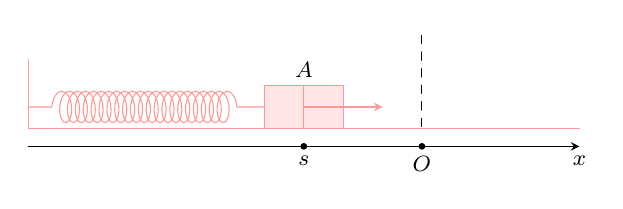
\begin{tikzpicture}[scale=1,font=\footnotesize, line join=round, line cap=round, >=stealth]
			\draw[red!40] (0,.6)--(0,-.27)--(7,-.27);
			\draw[red!40,fill=red!10] (3,-0.27) rectangle (3.5,.27) (3.5,-0.27) rectangle (4,.27);
			\draw[red!40,->] (3.5,0)--(4.5,0);
			\draw[red!40]
			[
			decoration={
				coil,
				segment length = 1mm,
				amplitude = 2mm,
				aspect = 0.5,
				post length = 3mm,
				pre length = 3mm},
			decorate] (0,0) -- ++(3,0);
			\draw[,->] (0,-.5) -- (7,-.5)node[below] {$x$};
			\draw[fill=black] 
			(3.5,-.5) circle (1pt) node[below] {$s$}
			(5,-.5) circle (1pt) node[below] {$O$}
			(3.5,.25) node[above] {$A$}
			;
			\draw[dashed] (5,-0.25)--(5,1);
			%%\path ([xshift=-.25cm]current bounding box.south) node[below]{\hinhve};
		\end{tikzpicture}
	\end{center}
	\shortans{$32$}
	\loigiai{
		Theo giả thiết, ta có 
		\allowdisplaybreaks
		\begin{eqnarray*}
			&&10 \sin \left(10 t+\dfrac{\pi}{2}\right)=-5\sqrt{3}
			\Leftrightarrow  \sin \left(10 t+\dfrac{\pi}{2}\right)=-\dfrac{\sqrt{3}}{2}\\
			&\Leftrightarrow & \sin \left(10 t+\dfrac{\pi}{2}\right)=\sin\left(-\dfrac{\pi}{3}\right)
			\Leftrightarrow \hoac{&10t+\dfrac{\pi}{2}=-\dfrac{\pi}{3}+k2\pi \\&10 t+\dfrac{\pi}{2}=\pi+\dfrac{\pi}{3}+l2\pi \\} \\
			&\Leftrightarrow &\hoac{&t=-\dfrac{\pi}{12}+\dfrac{k\pi}{5} \\&t=\dfrac{\pi}{12}+\dfrac{l\pi}{5} \\} (k, l\in \mathbb{Z}).
		\end{eqnarray*}
		Vậy để $s=-5\sqrt{3}$ cm thì $t=-\dfrac{\pi}{12}+\dfrac{k\pi}{5}$, $(k \in \mathbb{N}^*)$ và $t=\dfrac{\pi}{12}+\dfrac{l\pi}{5}$, $(l\in \mathbb{N})$. \\
		Xét $\hoac{&0\leq -\dfrac{\pi}{12}+\dfrac{k\pi}{5}\leq 10 \\ 
			&0\leq \dfrac{\pi}{12}+\dfrac{l\pi}{5}\leq 10}
		\Leftrightarrow \hoac{&\dfrac{5}{12}\leq k\leq \dfrac{50}{\pi}+\dfrac{5}{12}
			\rightarrow k\in \{1; 2; \ldots; 16\} \\ 
			&-\dfrac{5}{12}\leq l\leq \dfrac{50}{\pi}-\dfrac{5}{12}\rightarrow l\in \{0; 1; 2; \ldots; 15\}.}$\\
		Vậy trong $10$ giây đầu tiên, vật đi qua vị trí $s=-5\sqrt{3}$ cm $32$ lần.
	}
\end{ex}
\begin{ex}%[1D2V2-7]
	Chu vi của một đa giác bằng $158$ cm; các cạnh của đa giác lập thành một cấp số cộng với công sai $3$ cm. Biết cạnh dài nhất là $44$ cm. Số cạnh của đa giác đó bằng
	\shortans{$4$}
\loigiai{
	Gọi số cạnh đa giác là $n$ và các cạnh lần lượt là $u_1; u_2;\ldots; u_n$. \\
	Theo đề ra, ta có $u_n=44 \Leftrightarrow u_1+(n-1)d=44 \Leftrightarrow u_1=47-3n$.
	\begin{eqnarray*}
		&&S_n=\dfrac{u_1+u_n}{2}\cdot n \Leftrightarrow 158=\dfrac{91-3n}{2}\cdot n
		\Leftrightarrow 3n^2-91n+316=0 \Leftrightarrow \hoac{&n=4 \text{ (nhận)} \\ &n=\dfrac{79}{3} \text{ (loại).}}
	\end{eqnarray*}
	Vậy đa giác có $4$ cạnh.
}
\end{ex}
\begin{ex}%[1D2V3-8]
	Anh An muốn gửi tiết kiệm để cho con học đại học nên đầu mỗi tháng người này gửi ngân hàng $5$ triệu đồng. Sau khi gửi được $1$ năm, do cần tiền nên anh An đã rút hết tiền tiết kiệm ra để sử dụng. Hỏi anh An nhận được bao nhiêu triệu đồng? Biết lãi suất mỗi tháng là $0{,}7\%$. (Làm tròn đến số thập phân thứ nhất).
	\shortans{$62{,}8$}
\loigiai{
	Thiết lập công thức sau mỗi tháng, ta được
	\begin{itemize}
		\item Sau $1$ tháng được $5+5\cdot 0{,7}\%=5\left(1+0{,}7\%\right)$ (triệu đồng).
		\item Sau $2$ tháng được $5\left[\left(1+0{,}7\%\right)+\left(1+0{,}7\%\right)^2\right]$ (triệu đồng).
		\item $\ldots\ldots$
		\item Sau $n$ tháng, ta được $5\sum\limits_{i=1}^{n}\, \left(1+0{,}7\%\right)^i$ (triệu đồng).
	\end{itemize}
	Như vậy sau khi gửi được $12$ tháng, anh An được số tiền là
	\begin{eqnarray*}
		&&5\sum\limits_{i=1}^{12}\, \left(1+0{,}7\%\right)^i
		=5\cdot \left(1+0{,}7\%\right)\cdot \dfrac{\left(1+0{,}7\%\right)^{12}-1}{\left(1+0{,}7\%\right)-1}\approx 62{,}8 \text{ (triệu đồng).}
	\end{eqnarray*}
}
\end{ex}
\begin{ex}%[1D3V3-3]
	Cho hàm số $f(x)=\heva{\dfrac{x^2+x-6}{\sqrt{x+2}-\sqrt{3x-2}}&\text{ khi } x>2 \\ (2x-3)^2+a&\text{ khi } x\leq2}$. Với giá trị nào của $a$ thì hàm số liên tục trên $\mathbb{R}$?
	\shortans{$-11$}
\loigiai{
	Với $x>2$, ta có $f(x)=\dfrac{x^2+x-6}{\sqrt{x+2}-\sqrt{3x-2}}$ liên tục. \\
	Với $x<2$, ta có $f(x)=(2x-3)^2+a$ liên tục. \\
	Tại $x=2$, ta có
	\begin{itemize}
		\item $\lim\limits_{x\to 2^-}\, f(x)=f(2)=1+a$.
		\item $\lim\limits_{x\to 2^+} f(x)=\lim\limits_{x\to 2^+} \dfrac{x^2+x-6}{\sqrt{x+2}-\sqrt{3x-2}}
		=\lim\limits_{x\to 2^+} \dfrac{(x+3)(x-2)\left(\sqrt{x+2}+\sqrt{3x-2}\right)}{-2(x-2)}~{=-10}$.
	\end{itemize}
	Hàm số liên tục trên $\mathbb{R}$ khi $1+a=-10 \Leftrightarrow a=-11$.
}
\end{ex}
\begin{ex}%[1H4V6-5]
	Cho hình chóp $S.ABCD$ đáy là hình bình hành, $O$ là tâm của đáy. Trên cạnh $SB$, $SD$ lần lượt lấy điểm $M; N$ sao cho $SM=2MB$ và $SN=\dfrac{1}{3}SD$. Hình chiếu của $M; N$ qua phép chiếu song song đường thẳng $SO$ lên mặt phẳng chiếu $(ABCD)$ lần lượt là $P; Q$. Tính tỉ số $\dfrac{OP}{OQ}$.
	\shortans{$2$}
\loigiai{
	\begin{center}
		\begin{tikzpicture}[scale=1,line cap=round,line join=round,font=\footnotesize,>=stealth]
			\path (0,0) coordinate (A)++(0:4) coordinate (B)++(-130:2)coordinate (C)
			($(A)!.5!(C)$) coordinate (O)++(110:4) coordinate (S)
			($(O)!-1!(B)$) coordinate (D)
			($(S)!2/3!(B)$) coordinate (M) ($(S)!1/3!(D)$) coordinate (N)
			($(O)!2/3!(B)$) coordinate (P) ($(O)!1/3!(D)$) coordinate (Q);
			\draw[dashed] (D)--(A)--(B)--cycle
			(S)--(A)--(C) (S)--(O)
			(M)--(P) (N)--(Q)
			;
			\draw (S)--(B)--(C)--(D)--cycle
			(S)--(C);
			\foreach \a/\b in {A/170,B/0,C/-30,D/200,O/-90,S/40,M/50,N/130,P/-90,Q/-90}{
				\fill[draw=black] (\a)circle(.7pt) ($(\a)+(\b:2mm)$)node[scale=.8]{$\a$};
			}
		\end{tikzpicture}
	\end{center}
	\begin{itemize}
		\item Do $P$ là hình chiếu của $M$ qua phép chiếu song song với phương $SO$ nên ta có
		$MP\parallel SO \Rightarrow \dfrac{BM}{BS}=\dfrac{BP}{BO}=\dfrac{1}{3}
		\Rightarrow \dfrac{OP}{OB}=\dfrac{2}{3}\cdot$
		\item Tương tự, ta có $\dfrac{OQ}{OD}=\dfrac{1}{3}\cdot$
	\end{itemize}
	Ta được $\dfrac{OP}{OQ}=\dfrac{OP:OB}{OQ:OD}=2$ (do $OB=OD$).
}
\end{ex}
\begin{ex}%[1D5V1-4]
	Hãy sử dụng dữ liệu ở để tư vấn cho đại lí bảo hiểm xác định khách hàng nam ở tuổi nào hay mua bảo hiểm nhất. Số khách hàng mua bảo hiểm ở từng độ tuổi được thống kê như sau:
	\begin{center}
		\begin{tabular}{|l|c|c|c|c|c|}
		\hline 
			Độ tuổi & $[20 ; 30)$ & $[30 ; 40)$ & $[40 ; 50)$ & $[50 ; 60)$ & $[60 ; 70)$ \\
		\hline 
			Số khách hàng nam & $4$ & $6$ & $10$ & $7$ & $3$ \\
		\hline 
%			Số khách hang nữ & $3$ & $9$ & $6$ & $4$ & $2$ \\
%		\hline
	\end{tabular}
	\end{center}
	\shortans{$46$}
\loigiai{
	Nhóm chứa mốt của mẫu số liệu khách hàng nam là $[40; 50)$.\\
	Do đó $u_m=40, n_{m-1}=6; n_{m+1}=7; u_{m+1}-u_m=50-40=10$.\\
	Mốt của mẫu số liệu nhóm khách hàng nam là
	$M_0=40+\dfrac{10-6}{(10-6)+(10-7)} \cdot 10=45{,}7$.\\
	Dựa vào kết quả trên ta có thể dự đoán được khách hàng nam $46$ tuổi có nhu cầu mua bảo hiểm cao nhất.
%	Nhóm chứa mốt của mẫu số liệu khách hàng nữ là $[30; 40)$.\\
%	Do đó $u_m=30, n_{m-1}=3; n_{m+1}=6; u_{m+1}-u_m=40-30=10$.\\
%	Mốt của mẫu số liệu nhóm khách hàng nam là
%	$M_0=30+\dfrac{9-3}{(9-3)+(9-6)} \cdot 10=36{,}7$.\\
%	Dựa vào kết quả trên ta có thể dự đoán được khách hàng nữ $37$ tuổi có nhu cầu mua bảo hiểm cao nhất.
}
\end{ex}

